\chapter{Reproduction Guide}

Every quantitative result in this thesis is regenerated from a fixed
seed by a single script. Two classes of script must be distinguished.
Most are \emph{self-contained}: they generate their own synthetic
instances and run as-is on a clean checkout. The rest (the real-graph
and real-trace results of Chapters 7, 8 and 9) first need external data
placed under \path|data/|; that data is not redistributed with the
code, and §A.5 records what each dataset is and where it comes from. In
the map below, a dagger (\(\dagger\)) marks the scripts of the second
class.

This appendix maps each figure and table to its script, gives the
commands and runtimes, lists the full Phase-2 reproduction tables
deferred from Chapter 3, and records data provenance.

\section{Environment and principles}

\begin{itemize}
\tightlist
\item
  \textbf{Stack:} Python 3.12; NumPy 1.26+, SciPy 1.13, NetworkX 3.3,
  Matplotlib (plots only).
\item
  \textbf{Determinism:} all randomness derives from one master seed
  (default \path|0|) via NumPy's \path|default_rng(seed).spawn(k)|,
  which yields independent, reproducible streams (graph, instance,
  algorithm randomness, prediction perturbation). Results are bit-stable
  across NumPy minor versions from 1.25 (BitGenerator-based spawning).
\item
  \textbf{Paired trials:} within a comparison, every algorithm and error
  level reuses the same graph, arrival sequence, \path|OPT|, and
  tie-break seed, so differences are attributable to the prediction
  alone.
\item
  \textbf{Confidence intervals:} 95\% normal-approximation half-widths
  over trials.
\item
  \textbf{Flow decompositions.} Three preprocessing steps (Feldman,
  Jaillet--Lu, and the serving advice \(b\)-matching) take a maximum
  flow and consume its \emph{decomposition}, which, unlike the flow
  value, is not unique. Their networks label nodes with integers rather
  than strings, so that the decomposition NetworkX returns is stable
  from run to run; with string labels it followed Python's per-process
  string hashing and every number derived from it moved between runs of
  the same script.
\item
  Each script writes \texttt{results/\textless{}name\textgreater{}.json}
  (raw means/CIs) and \texttt{results/\textless{}name\textgreater{}.png}
  (plot), and prints per-step progress.
\end{itemize}

\section{\texorpdfstring{Figure / table \ensuremath{\rightarrow} script
map}{Figure / table  script map}}

{ % do not increment counter
\footnotesize
\linespread{1}\selectfont
\setlength{\tabcolsep}{3pt}
\begin{longtable}[]{@{}
  >{\raggedright\arraybackslash}p{(\linewidth - 6\tabcolsep) * \real{0.2400}}
  >{\raggedright\arraybackslash}p{(\linewidth - 6\tabcolsep) * \real{0.2900}}
  >{\raggedright\arraybackslash}p{(\linewidth - 6\tabcolsep) * \real{0.3400}}
  >{\raggedright\arraybackslash}p{(\linewidth - 6\tabcolsep) * \real{0.1300}}@{}}
\toprule\noalign{}
\begin{minipage}[b]{\linewidth}\raggedright
Thesis object
\end{minipage} & \begin{minipage}[b]{\linewidth}\raggedright
Script
\end{minipage} & \begin{minipage}[b]{\linewidth}\raggedright
Output
\end{minipage} & \begin{minipage}[b]{\linewidth}\raggedright
\(\approx\) runtime
\end{minipage} \\
\midrule\noalign{}
\endhead
\bottomrule\noalign{}
\endlastfoot
Fig 3.1 (ER U-curve) & \path|scripts/run_er_full.py| &
\path|results/er_full.{json,png}| & \textasciitilde20 min \\
Fig 3.2 (left-regular) & \path|scripts/run_left_regular.py| &
\path|results/left_regular.{json,png}| & \textasciitilde10 min \\
§3.1 / §3.5 methodology checks & \path|scripts/run_metric_check.py|
& \path|results/metric_check.json| & \textasciitilde90 s \\
\textbf{Table 4.1} (unified benchmark) &
\path|scripts/run_unified_benchmark.py|, then
\path|plot_unified_panels.py| &
\path|results/unified_benchmark.{json,png}|,
\path|unified_benchmark_panel{A,B,C}.png|,
\path|unified_benchmark_tables.md| & \textasciitilde100 s \\
Fig 4.1 (consistency--robustness plane) &
\path|scripts/run_consistency_robustness.py| &
\path|results/consistency_robustness.{json,png}| & \textasciitilde1
s \\
Fig 5.1 (order-error vs ACI) &
\path|scripts/run_order_vs_theory.py| &
\path|results/order_vs_theory.{json,png}| & \textasciitilde30 s \\
Fig 6.1 (envelope), Fig 6.2 (prefix sweep) &
\path|scripts/run_choo_bem.py| &
\path|results/choo_bem_{envelope,prefix}.png| & \textasciitilde20
min \\
Fig 6.3, recalibration (§6.3) & \path|scripts/run_recalibration.py| &
\path|results/recalibration_*.png| & \textasciitilde1.5 min \\
Fig 6.4 (testing-wall frontier) &
\path|scripts/run_impossibility_frontier.py| &
\path|results/impossibility_frontier.{json,png}| & \textasciitilde6
s \\
Fig 7.1 (real predictor) \(\dagger\) &
\path|scripts/run_real_predictor.py| &
\path|results/real_predictor.{json,png}| & \textasciitilde15 s \\
Fig 7.2 (six real graphs) \(\dagger\) &
\path|scripts/run_realworld_robustness.py| &
\path|results/realworld_robustness.{json,png}| & \textasciitilde65
s \\
Fig 8.1 (M0 rank vs MSE) & \path|scripts/run_rank_vs_mse_mve.py| &
\path|results/rank_vs_mse_mve.{json,png}| & \textasciitilde10
s \\
M1 sweep (§8.1, no figure) &
\path|scripts/run_rank_when_it_matters.py| &
\path|results/rank_when_it_matters.{json,png}| &
\textasciitilde20 s \\
Fig 8.2 (M3 real-trace learning) \(\dagger\) &
\path|scripts/run_rank_real_trace.py| &
\path|results/rank_real_trace.{json,png}| & \textasciitilde10 s \\
Fig 8.3 (serving SLO probe) &
\path|scripts/run_serving_slo_probe.py| &
\path|results/serving_slo_probe.{json,png}| & \textasciitilde1
s \\
Figs 9.1--9.3, serving (Ch 9) \(\dagger\) &
\path|scripts/run_serving.py|, \path|run_serving_trace.py|,
\path|run_serving_dynamic.py|, \path|run_prefix_cache.py| &
\path|results/serving_*.png|, \path|prefix_cache_*.png| &
varies \\
Ladder, streaming (§A.7) & \path|scripts/run_streaming_ladder.py|,
then \path|plot_streaming_ladder.py| &
\path|results/streaming_ladder.{json,png}|,
\path|streaming_ladder_tables.md| & \textasciitilde40 s \\
Outlook checks (§A.6) & \path|scripts/verify_witness_gap.py| &
console output & seconds \\
Real-world Borodin Tables 3/4 (validation) \(\dagger\) &
\path|scripts/run_realworld.py| & \path|results/realworld.json| &
\textasciitilde few min \\
\end{longtable}
}

Runtimes are wall-clock on one machine (Apple M4 Pro, 12 cores); the
scripts are single-threaded apart from NumPy's own vectorization, so
they scale with single-core speed.

\textbf{Interval convention (deferred from §3.5).}
\path|run_metric_check.py| also compares the per-algorithm
confidence intervals the thesis reports against paired-difference
intervals on the same trials. Where the per-instance ratios are
positively correlated the paired interval is \(1.7\)--\(2.6\times\)
narrower (correlations \(0.67\) and \(0.85\)); where they are not (blind
following against Ranking under garbage advice, correlation \(-0.15\))
pairing does not help and the per-algorithm interval is the honest one.
The narrowest margin in the thesis, Feldman(MPD)'s \(+0.0044\) against a
\(\pm0.0023\) per-algorithm interval, tightens to \(\pm0.0009\) under
pairing.

\section{Reproduction commands}

{\footnotesize\linespread{1}\selectfont
\begin{verbatim}
# from the project root (matching-experiments/)
# correctness anchors: 8 hand-verifiable test files, all pass:
for t in tests/test_*.py; do python3 "$t"; done

# regenerate the headline results (fast ones):
python3 scripts/run_unified_benchmark.py        # Table 4.1 (data)
python3 scripts/plot_unified_panels.py          # Table 4.1 (panel charts; needs the line above)
python3 scripts/run_order_vs_theory.py          # Fig 5.1
python3 scripts/run_real_predictor.py           # Fig 7.1
python3 scripts/run_realworld_robustness.py     # Fig 7.2
python3 scripts/run_impossibility_frontier.py   # Fig 6.4
python3 scripts/run_rank_vs_mse_mve.py          # Fig 8.1
python3 scripts/run_rank_when_it_matters.py     # M1 (§8.1)
python3 scripts/run_rank_real_trace.py          # Fig 8.2
python3 scripts/run_serving_slo_probe.py        # Fig 8.3
python3 scripts/run_consistency_robustness.py   # Fig 4.1 (needs run_unified_benchmark first)
python3 scripts/run_metric_check.py             # §3.1 and §3.5 methodology checks
python3 scripts/run_streaming_ladder.py         # §A.7 ladder (data)
python3 scripts/plot_streaming_ladder.py        # §A.7 figure (needs the line above)

# the long (max-flow / Hopcroft–Karp-bound) sweeps:
python3 scripts/run_er_full.py                  # Fig 3.1  (~20 min)
python3 scripts/run_left_regular.py             # Fig 3.2  (~10 min)
python3 scripts/run_choo_bem.py                 # Fig 6.1, 6.2 (~20 min)
\end{verbatim}
}

All scripts hardcode seed \path|0| unless noted; re-running reproduces
the reported numbers.

\section{Full Phase-2 reproduction tables (deferred from
§3.6)}

Setup: \(n=1000\), \(m=n\), 100 trials per parameter value, seed 0.
Target is \emph{qualitative} agreement with Borodin et
al.~(Python/NetworkX vs the paper's C++/Edmonds--Karp; absolute
differences \(\le 0.02\) accepted).

\textbf{Erdős--Rényi, competitive ratio at selected \(c\)}
(SG=SimpleGreedy, Rk=Ranking, F/J = Feldman/Jaillet--Lu, -NG/-G =
non-greedy/greedy):

{ % do not increment counter
\begin{longtable}[]{@{}rrrrrrr@{}}
\toprule\noalign{}
\(c\) & SG & Rk & F-NG & F-G & J-NG & J-G \\
\midrule\noalign{}
\endhead
\bottomrule\noalign{}
\endlastfoot
0.10 & 1.000 & 0.999 & 1.000 & 1.000 & 0.999 & 1.000 \\
1.90 & 0.936 & 0.936 & 0.904 & 0.964 & 0.920 & 0.961 \\
\textbf{4.90} & \textbf{0.864} & 0.866 & 0.764 & \textbf{0.884} & 0.795
& \textbf{0.886} \\
8.90 & 0.909 & 0.909 & 0.730 & 0.912 & 0.765 & 0.913 \\
14.90 & 0.949 & 0.949 & 0.730 & 0.949 & 0.760 & 0.948 \\
\end{longtable}
}

Per-algorithm minima (ER): SG 0.864 @ \(c\)=4.9; Rk 0.865 @ 4.7; F-NG
0.728 @ 14.5; F-G 0.884 @ 5.3; J-NG 0.759 @ 13.9; J-G 0.884 @ 5.3.

\textbf{Random left-regular, competitive ratio at selected \(d\):}

{ % do not increment counter
\begin{longtable}[]{@{}rrrrrrr@{}}
\toprule\noalign{}
\(d\) & SG & Rk & F-NG & F-G & J-NG & J-G \\
\midrule\noalign{}
\endhead
\bottomrule\noalign{}
\endlastfoot
1 & 1.000 & 1.000 & 0.985 & 1.000 & 0.985 & 1.000 \\
2 & 0.954 & 0.954 & 0.877 & 0.968 & 0.894 & 0.966 \\
\textbf{5} & \textbf{0.890} & 0.890 & 0.758 & 0.900 & 0.788 & 0.901 \\
10 & 0.927 & 0.928 & 0.733 & 0.928 & 0.766 & 0.928 \\
30 & 0.977 & 0.977 & 0.730 & 0.976 & 0.760 & 0.976 \\
\end{longtable}
}

\textbf{Paper-claim checklist (all verified \(\checkmark\)):} greedy
minima near \(c\approx4.9\) / \(d=5\); Ranking \(\approx\) SimpleGreedy
(max diff 0.0017 ER, 0.0013 LR; the paper omits Ranking's curve for this
reason); non-greedy variants degrade monotonically as \(c,d\) grow;
greedy complex variants \(\approx\) SimpleGreedy asymptotically; the
\(c\)=14.9 non-greedy ordering (J-NG 0.760 \textgreater{} F-NG 0.730)
matches the paper's worst-case-bound ordering. Across families, the
non-greedy algorithms converge to the same asymptotic constants (0.730
Feldman, 0.760 Jaillet--Lu, within 0.001), above their worst-case bounds
by +0.06 / +0.03; §3.6 reads that observation.

\section{Data provenance}

Real data is stored locally under \path|data/| (large; excluded from
version control).

\begin{itemize}
\tightlist
\item
  \textbf{Real graphs (Chapter 7, §3.6 validation):} six graphs from the
  Network Repository (\path|networkrepository.com|):
  \path|socfb-Caltech36|, \path|socfb-Reed98|, \path|bio-CE-GN|,
  \path|bio-CE-PG|, \path|econ-beause|, \path|econ-mbeaflw|,
  downloaded as MatrixMarket \path|.mtx| / whitespace \path|.edges|,
  reduced to simple undirected graphs and converted to bipartite by
  random balanced partition (Borodin Table 3) or duplicating
  double-cover (Table 4).
\item
  \textbf{Traces (Chapters 7, 8, 9):} Wikipedia ``top articles per day''
  for four days, retrieved from the Wikimedia REST pageviews API
  (\path|data/trace/wiki/|, used as live day vs 1/7/30-day-stale
  forecasts); the Azure LLM inference trace from Microsoft's public
  Azure dataset release (\path|data/trace/azure_llm/|,
  context/generated token counts with timestamps); and the Mooncake
  conversation trace released with \autocite{mooncake2024}
  (\path|data/trace/mooncake/|, per-request \path|hash_ids| for
  prefix-cache blocks). The Wikipedia trace is a snapshot of a live
  source rather than a static benchmark, so exact reproduction needs the
  same snapshot, not merely the same API.
\end{itemize}

\section{Outlook verification snippets
(§10.2)}

Every quantity quoted in the outlook of §10.2 was checked numerically
before being used. There are three checks, each a short simulation of
the rare-resource construction.

\begin{enumerate}
\def\labelenumi{\arabic{enumi}.}
\tightlist
\item
  \textbf{Per-cell constants.} The per-cell optimum, the per-cell
  baseline, and the closed forms for the advantage and for \(\ell_1\)
  agree with simulation to three decimals. For example, at contention
  \(\theta=0.6\) and advice bias \(0.3\) the simulated per-cell
  advantage is \(\pm0.119\), against a predicted
  \(\pm\theta\cdot0.3 = \pm0.12\).
\item
  \textbf{The conversion law.} The expected ratio when the advice is
  followed matches \(\rho_{\mathrm{perfect}} - \tfrac12\ell_1(p,q)\),
  where \(\rho_{\mathrm{perfect}}\) is the ratio under perfect advice,
  i.e.~it falls off linearly in the advice's \(\ell_1\) error, again to
  three decimals. In the language of §10.2 this is what makes the
  \emph{stakes} \(\delta\) a linear function of the advice error.
\item
  \textbf{The two budget--stakes ingredients.} The directional
  statistic's accuracy at a fixed prefix length does not degrade as
  \(n\) grows, and the plug-in \(\ell_1\) estimate becomes blind,
  i.e.~indistinguishable between good and bad advice, once \(k \ll r\).
  Both are produced by \path|scripts/verify_witness_gap.py| (§A.2).
\end{enumerate}

These checks are what license the \emph{reading} of §10.2; they are not
a proof of it. The formal development is separate work outside this
thesis.

\section{The relaxation ladder: streaming and offline
algorithms}

The original project brief suggested extending the reproduction with
\emph{streaming or offline algorithms}. My proposal instead made the
learning-augmented family the main extension. This appendix supplies the
suggested arm at reduced scope and connects it to the thesis's central
question: is the small remaining gap to the optimum caused by missing
information, or by the irrevocability of online decisions?

The comparison is a \textbf{ladder of relaxations} on the same
instances. Online vertex arrival reveals one node's neighbourhood at a
time and requires an immediate, irrevocable match. The semi-streaming
variant instead receives edges in a uniformly random order and stores
only \(O(n)\) words. Its first pass is greedy; each additional pass
applies vertex-disjoint length-3 augmentations
\autocite{feigenbaum2005semistreaming,mcgregor2005matchings}. The
offline rung is the Hopcroft--Karp optimum already used as the
denominator throughout the thesis. This is not a claim that streaming is
an online algorithm: extra passes explicitly relax irrevocability.

\textbf{Setup.} The ladder uses the three synthetic families of Table
4.1 and the six real graphs of §7.2, with the same instances, optimum
and \(95\%\) interval convention. Its online rows reproduce Table 4.1
within the reported intervals. Full numerical outputs are in
\path|results/streaming_ladder_tables.md|; Figure A.1 shows the four
rungs needed for the comparison.

\begin{figure}
\centering
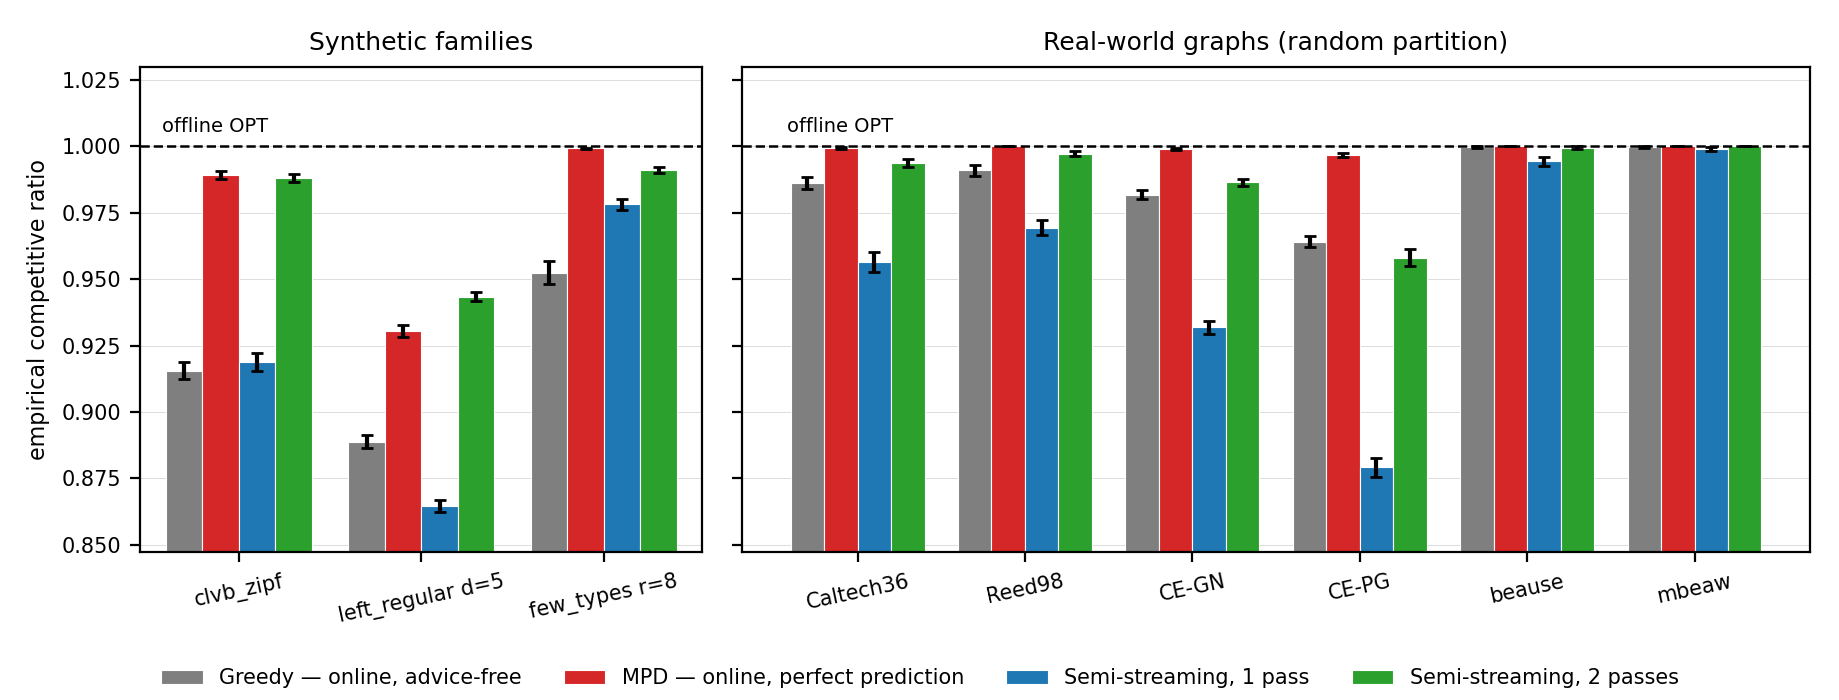
\includegraphics[width=0.85\linewidth,height=\textheight,keepaspectratio,alt={The relaxation ladder. Grey and red are the online model (advice-free Greedy, and MPD given a perfect degree prediction); blue and green are semi-streaming at one and two passes. On seven of the nine graphs one extra pass buys more than a perfect prediction does.}]{../../results/streaming_ladder.png}
\caption{The relaxation ladder. Grey and red are the online model
(advice-free Greedy, and MPD given a perfect degree prediction); blue
and green are semi-streaming at one and two passes. On seven of the nine
graphs one extra pass buys more than a perfect prediction does.}
\end{figure}

The important comparison is marginal. Perfect degree advice improves the
online baseline; one revision pass improves the one-pass streaming
baseline. One revision is worth more than perfect advice on seven of the
nine graphs, including all six real ones. It lifts every graph to within
\(0.6\)--\(4.2\%\) of the optimum. The exceptions are
\path|clvb_zipf|, where the gains differ by less than \(0.005\), and
\path|few_types|, the synthetic family deliberately constructed to
reward degree information. Thus, on these average-case inputs, the
residual gap is more responsive to revision than to better prediction.
This supports the thesis's interpretation that prediction has little
performance headroom because the advice-free baseline is already strong;
the remaining loss is largely the price of irrevocability rather than an
information deficit.

The comparison is deliberately limited. Because dispatched decisions
cannot be recalled, the second pass is unavailable in the motivating
applications; the experiment compares the \emph{size} of the two gains,
not their practical interchangeability. It tests one simple family under
random rather than adversarial edge order, without stronger
\((1-\varepsilon)\)-approximation streaming algorithms. It is evidence
about where the gap lies, not a full benchmark.
